\part{Correction of Software Systems}\mypartpage
%%%%%%%%%%%%%%%%%%%%%%%%%%%%%%%%%%%%%%%%%%%%%%%%%%%%%%%%%%%%%%%%%%%%%%%%%% 
\section{Introduction}
\begin{frame}{Sorting Algorithm Performance Discussion}
  \begin{block}<+->{We have shown that}\medskip

    \begin{tabular}{|l|c|c|c|c|}\cline{2-5}
      \multicolumn{1}{}{}&
        \multicolumn{3}{|c|}{\structure{Amount of comparisons}}&
        \structure{Memory}\\\cline{2-4}
      \multicolumn{1}{c|}{}&\structure{Best Case}&
        \structure{Average Case}&\structure{Worst Case}&
        \structure{Complexity}\\\hline

      Selection Sort&$O(n^2)$&$O(n^2)$&$O(n^2)$&$\Theta(1)$\\\hline
      Insertion Sort&$O(n)$&$O(n^2)$&$O(n^2)$&$\Theta(1)$\\\hline
      Bubble Sort&$O(n)$&$O(n^2)$&$O(n^2)$&$\Theta(1)$\\\hline 

      \hline
      Quick Sort&$O(n\log(n))$&$O(n\log(n))$&$O(n^2)$&$O(\log(n))$\\\hline
      Merge Sort&$O(n\log(n))$&$O(n\log(n))$&$O(n\log(n))$&$O(n)$\\\hline      
    \end{tabular}

    \begin{itemize}
    \item Very accurate knowledge on achieved performance
    \end{itemize}
  \end{block}

  \visible<+->{
  \concept{But wait a second\ldots}
  
  \begin{block}{How do you know this code actually sorts the array?}
    \begin{itemize}
    \item Because you see it, it's obvious (yeah, right\ldots)
    \item Because the teacher / a friend says so
    \item Because it's written in a book / on the Internet
    \item Because you tested it
    \end{itemize}
  \end{block}
}
\end{frame}  
%%%%%%%%%%%%%%%%%%%%%%%%%%%%%%%%%%%%%%%%%%%%%%%%%%%%%%%%%%%%%%%%%%%%%%%%%%%%
\begin{frame}{Because it's obvious you said?}
  \begin{block}{Let's consider the following problem}
    \begin{itemize}
    \item You have a robot arm equipped with a soldering iron (for example)
    \item You have several positions were the arm should do its soldering job
    \item You must decide the order in which the arm visit the positions
    \item You want to minimize the time (ie travel distance) it takes to visit
      all positions
    \end{itemize}
  \end{block}

  \centerline{\includegraphics[width=.6\linewidth]{fig/proof_salesman1.fig}}
\end{frame}
%%%%%%%%%%%%%%%%%%%%%%%%%%%%%%%%%%%%%%%%%%%%%%%%%%%%%%%%%%%%%%%%%%%%%%%%%%%%%%
\begin{frame}{Nearest Neighbor Tour}
  \begin{block}{Here is a very popular algorithm to that problem}
    \begin{itemize}
    \item Pick and visit an initial point $p_0$, and let $i=0$
    \item While there are still unvisited points
      \begin{itemize}
      \item $i=i+1$
      \item let $p_i$ be the closest unvisited point to $p_{i-1}$
      \item Visit $p_i$
      \end{itemize}
    \item Return to $p_0$ from $p_i$
    \end{itemize}
  \end{block}

  \begin{block}{Advantage of that algorithm}
    \begin{itemize}
    \item It is simple to understand and implement; It's very efficient: $O(n)$
    \end{itemize}
  \end{block}
  
  \begin{alertblock}<2->{\only<2->{But it is not correct!}}
    \begin{minipage}{.6\linewidth}
      \only<1| handout:0>{\includegraphics[width=\linewidth,subfig=1]{fig/proof_salesman2.fig}}%
      \only<2| handout:0>{\includegraphics[width=\linewidth,subfig=2]{fig/proof_salesman2.fig}}%
      \only<3->{\includegraphics[width=\linewidth,subfig=3]{fig/proof_salesman2.fig}}%      
    \end{minipage}\hfill
    \begin{minipage}{.35\linewidth}
      \begin{center}
        \only<4>{Choosing carefully $p_0$\\
          (left-most or whatever) \\
          \alert{will \textbf{not} help}}        
      \end{center}
    \end{minipage}
  \end{alertblock}
\end{frame}
%%%%%%%%%%%%%%%%%%%%%%%%%%%%%%%%%%%%%%%%%%%%%%%%%%%%%%%%%%%%%%%%%%%%%%%%%% 
\begin{frame}{Closest Pair Tour}
  \begin{block}{Let's try to fix our algorithm}
    \begin{itemize}
    \item Walking to the closest point seems too restrictive: 
      {\small traps into unwanted moves}
    \item Let's repeatedly connect the closest pairs 
      {\small(w/o forming cycles or 3ways branches)}
    \end{itemize}
  \end{block}\vspace{-.8\baselineskip}

  \begin{block}{The algorithm}
    \begin{itemize}
    \item Let $n$ be the number of points in the set 
    \item For $i=1$ to $n-1$ do
      \begin{itemize}
      \item Let $d=\infty$
      \item For each pair of endpoints $(x,y)$ of partial paths
        \begin{itemize}
        \item If $dist(x,y)\leq d$ then $x_m=x$, $y_m=y$, $d=dist(x,y)$
        \end{itemize}
      \item Connect $(x_m,y_m)$ by an edge
      \end{itemize}
    \item Connect the two endpoints by an edge
    \end{itemize}
  \end{block}\vspace{-.7\baselineskip}

  \begin{block}{Works correctly for previous data\only<2->{, \alert{but still
          not correct}}}\medskip
    \begin{center}
      \only<1-2| handout:0>{\includegraphics[width=.6\linewidth,subfig=1]{fig/proof_salesman3.fig}}%
      \only<3| handout:0>{\includegraphics[width=.6\linewidth,subfig=2]{fig/proof_salesman3.fig}}%
      \only<4->{\includegraphics[width=.6\linewidth,subfig=3]{fig/proof_salesman3.fig}}%      
      
    \end{center}    
  \end{block}
\end{frame}
%%%%%%%%%%%%%%%%%%%%%%%%%%%%%%%%%%%%%%%%%%%%%%%%%%%%%%%%%%%%%%%%%%%%%%%%%% 
\begin{frame}{That's the Traveling Salesman Problem}
  \begin{block}{A correct algorithm}
    \begin{itemize}
    \item $d=\infty$
    \item For each permutation $\Pi_i$ of the $n!$ existing ones
      \begin{itemize}
      \item if ($cost(\Pi_i)\leq d$) then
        \begin{itemize}
        \item $d=cost(\Pi_i)$ and $P_{min}=\Pi_i$
        \end{itemize}
      \end{itemize}
    \item return $P_i$
    \end{itemize}
  \end{block}

  \begin{block}{Actually no known correct and polynomial algorithm}
    \begin{itemize}
    \item This algorithm is very slow (exponential time)
    \item But that's the only correct known
    \item (this problem is one of the NP-Complete set, by the way)
    \end{itemize}
  \end{block}

  \bigskip
  \concept{Conclusion: never trust ``obviously correct'' algorithms}
\end{frame}
%%%%%%%%%%%%%%%%%%%%%%%%%%%%%%%%%%%%%%%%%%%%%%%%%%%%%%%%%%%%%%%%%%%%%%%%%% 
\begin{frame}{Other try to convince septics: \alert{you test it}}
  \begin{block}{Issues} 
    \begin{itemize}
    \item a \textit{whole} load of arrays exists out there. Cannot test them
      all\ldots
     \item How much should you test to get convincing?
       Which ones do you pick?
   \end{itemize}
  \end{block}

  \begin{block}{Let's look at another (simpler) problem}
    \begin{itemize}
    \item \structure{Input:} 3 integers values, representing the sides'
      length of a triangle
    \item \structure{Output:} Tells whether the triangle is
      \begin{itemize}
      \item \structure{Scalene:} no two sides are equal
      \item \structure{Isosceles:} exactly two sides are equal
      \item \structure{Equilateral:} all sides are equal
      \end{itemize}
    \end{itemize}
  \end{block}

  \begin{alertblock}{Quiz: Create a set of Test Cases for this program}
    \begin{itemize}
    \item Ie, the list of tests you need to write to ensure that the program is robust
    \end{itemize}
  \end{alertblock}
\end{frame}
%%%%%%%%%%%%%%%%%%%%%%%%%%%%%%%%%%%%%%%%%%%%%%%%%%%%%%%%%%%%%%%%%%%%%%%%%% 
\begin{frame}[squeeze]{Solutions -- 1 point for each correct answer}
  \begin{itemize}
  \item T1: \trou{(4,1,2): Invalid triangle (because $(a,b,c)$ with $a>b+c$)%
      \hbox to 2cm{\vbox to.6\baselineskip{\includegraphics[scale=.5]{fig/proof_triangle1.fig}}}}%
  \item T2: \trou{Permutations of the previous: $(1,2,4)$, $(2,1,4)$~~~~~~~~~~~~~~~~~~~~~~~~~~~~~~~}
    \trou{$\leadsto$ valid iff $a\leq b+c$ 
      \textbf{and $\mathbf{b\leq a+c}$ and $\mathbf{c\leq a+b}$} ~~~~~~~~~~~~~~~~~~~~~~~~~~~~~~} 
  \item T3: \trou{Invalid with equal sum: $(4,2,2)$ $\leadsto$ need to use $<$
      instead of $\leq$~~~~~~~~~~~}
  \item T4: \trou{Permutations of the previous: $(2,4,2)$, $(2,2,4)$~~~~~~~~~~~~~~~~~~~~~~~~~~~~~~~}
  \item T5: \trou{A valid scalene triangle: $(3,4,5)$~~~~~~~~~~~~~~~~~~~~~~~~~~~~~~~~~~~~~~~~~~~~~~~~}
  \item T6: \trou{A valid equilateral triangle: $(3,3,3)$~~~~~~~~~~~~~~~~~~~~~~~~~~~~~~~~~~~~~~~~~~~~}
  \item T7: \trou{A valid isoceles triangle: $(3,4,3)$~~~~~~~~~~~~~~~~~~~~~~~~~~~~~~~~~~~~~~~~~~~~~~~}
  \item T8: \trou{All permutations of isoceles triangle: $(4,3,3)$,$(3,3,4)$~~~~~~~~~~~~~~~~~~~~~~}
  \item T9: \trou{One side with \textbf{zero} value: $(0,4,3)$~~~~~~~~~~~~~~~~~~~~~~~~~~~~~~~~~~~~~~~~~~~~}
  \item T10: \trou{One side with \textbf{negative} value: $(-1,4,3)$~~~~~~~~~~~~~~~~~~~~~~~~~~~~~~~~~~~~}
  \item T11: \trou{All sides with \textbf{zero} values: $(0,0,0)$~~~~~~~~~~~~~~~~~~~~~~~~~~~~~~~~~~~~~~~~~~~}
  \item T12: \trou{At least one side non-integer: $(1,3,2.6)$ or even $(1,2,a)$~~~~~~~~~~~~~~~~~}
  \item T13: \trou{Wrong number of arguments: $(2,4)$ or $(1,2,2,5)$~~~~~~~~~~~~~~~~~~~~~~~~~~}
  \end{itemize}
\end{frame}
%%%%%%%%%%%%%%%%%%%%%%%%%%%%%%%%%%%%%%%%%%%%%%%%%%%%%%%%%%%%%%%%%%%%%%%%%%%%
\begin{frame}{First Conclusions on Testing}
  \begin{block}{About the Quiz}
    \begin{itemize}
    \item All T1-T13 correspond to failures actually found in some implementations
    \item How many tests did you found yourself?\\
      $<5$? ~~ $5-7$? ~~ $8-10$? ~~ $>10$? ~~ All?
    \item Highly qualified, experienced programmers score \alert{7.8} on average
    \end{itemize}
  \end{block}
  \begin{block}{Testing aint easy}
    \begin{itemize}
    \item Finding good and sufficiently many test cases is difficult
    \item Even a good set of test cases cannot exclude \alert{all} failures
    \item Without a specification, it is not clear even what a failure
      \alert{is} 
    \end{itemize}
  \end{block}
\end{frame}
%%%%%%%%%%%%%%%%%%%%%%%%%%%%%%%%%%%%%%%%%%%%%%%%%%%%%%%%%%%%%%%%%%%%%%%%%%%%%
\begin{frame}{Stop academic examples, check Real Life!}
  \begin{block}{Cost of Software Errors: some numbers}
    \begin{itemize}
    \item \structure{\$60 billion}: Estimated cost of software errors for US
      economy per year [2002]
    \item \structure{\$240 billion}: Size of US software industry [2002]\\
      {\small incl. profit, sales, marketing, development (50\% maybe)}
    \item \structure{50\%}: estimated part of each software project spent on
      testing\\ 
      {\small(spans from 30\% to 80\%)}

    \item Rough estimate: \structure{money spent on testing $\approx$ cost of
        remaining errors}
    \item That's \alert{50\% of size of software industry!}
    \end{itemize}
  \end{block}

 \begin{block}{More on Testing in POO lecture, in january}
   \begin{itemize}
   \item We need \structure{systematic}, \structure{efficient}, \structure{tool
       supported} \alert{testing} and \alert{debugging} methods
   \end{itemize}
 \end{block}
  
 \begin{block}{To convince real septics, you have to \textbf{prove} correctness}
   \begin{itemize}
   \item And you cannot do that without a proper specification (at least)
   \end{itemize}
 \end{block}
\end{frame}
%%%%%%%%%%%%%%%%%%%%%%%%%%%%%%%%%%%%%%%%%%%%%%%%%%%%%%%%%%%%%%%%%%%%%%%%%% 
\section{Specification}\sectionpage
\begin{frame}{How to prove that 'selection sort' sorts arrays?}
  \begin{block}{Back to the roots: what exactly do you want to prove?}
    \begin{itemize}
    \item Proper specification mandatory to proof: gives what we have, what we
      want
    \item We also need a mathematical logic to carry the proof
    \end{itemize}
  \end{block}

  \begin{block}{Hoare Logic {\normalsize[Hoare 1969]}}
    \begin{itemize}
    \item Set of logical rules to reason about the correctness of computer
      programs
    \item \structure{Central feature:} description of state changes induced by
      code execution
    \item \alert{\textbf{Hoare triple:}} \framebox{$\{P\}~ C ~\{Q\}$}
      \begin{itemize}
      \item C is the code to be run
      \item P is the \alert{\textbf{precondition}}
        (assertion about previous state)
      \item Q is the \alert{\textbf{postcondition}}
        (assertion about next state)
      \item This can be read as ``If P is true, then when I run C, Q becomes
        true''
      \item C is said to satisfy specification $(P,Q)$
      \end{itemize}
    \item Such notation allows very precise algorithm specifications
    \item Axioms and Inference rules allow rigorous correctness demonstrations
      \smallskip
    \item \structure{Note:} other logics (temporal logic) proposed as
      replacement, but harder
    \end{itemize}
  \end{block}
\end{frame}
%%%%%%%%%%%%%%%%%%%%%%%%%%%%%%%%%%%%%%%%%%%%%%%%%%%%%%%%%%%%%%%%%%%%%%%%%%%%%%
\begin{frame}{Introducing (bad) joke about precise specification}
  \begin{block}{While traversing Scotland, 3 people see a cow}\medskip
    \begin{columns}
      \begin{column}{.55\linewidth}
        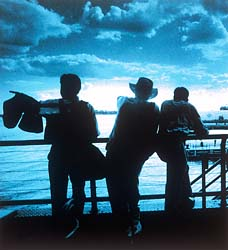
\includegraphics[width=.3\linewidth]{img/proof_guys.png}\hfill
        
\includegraphics[width=.6\linewidth]{img/proof_scotland.png}
        
        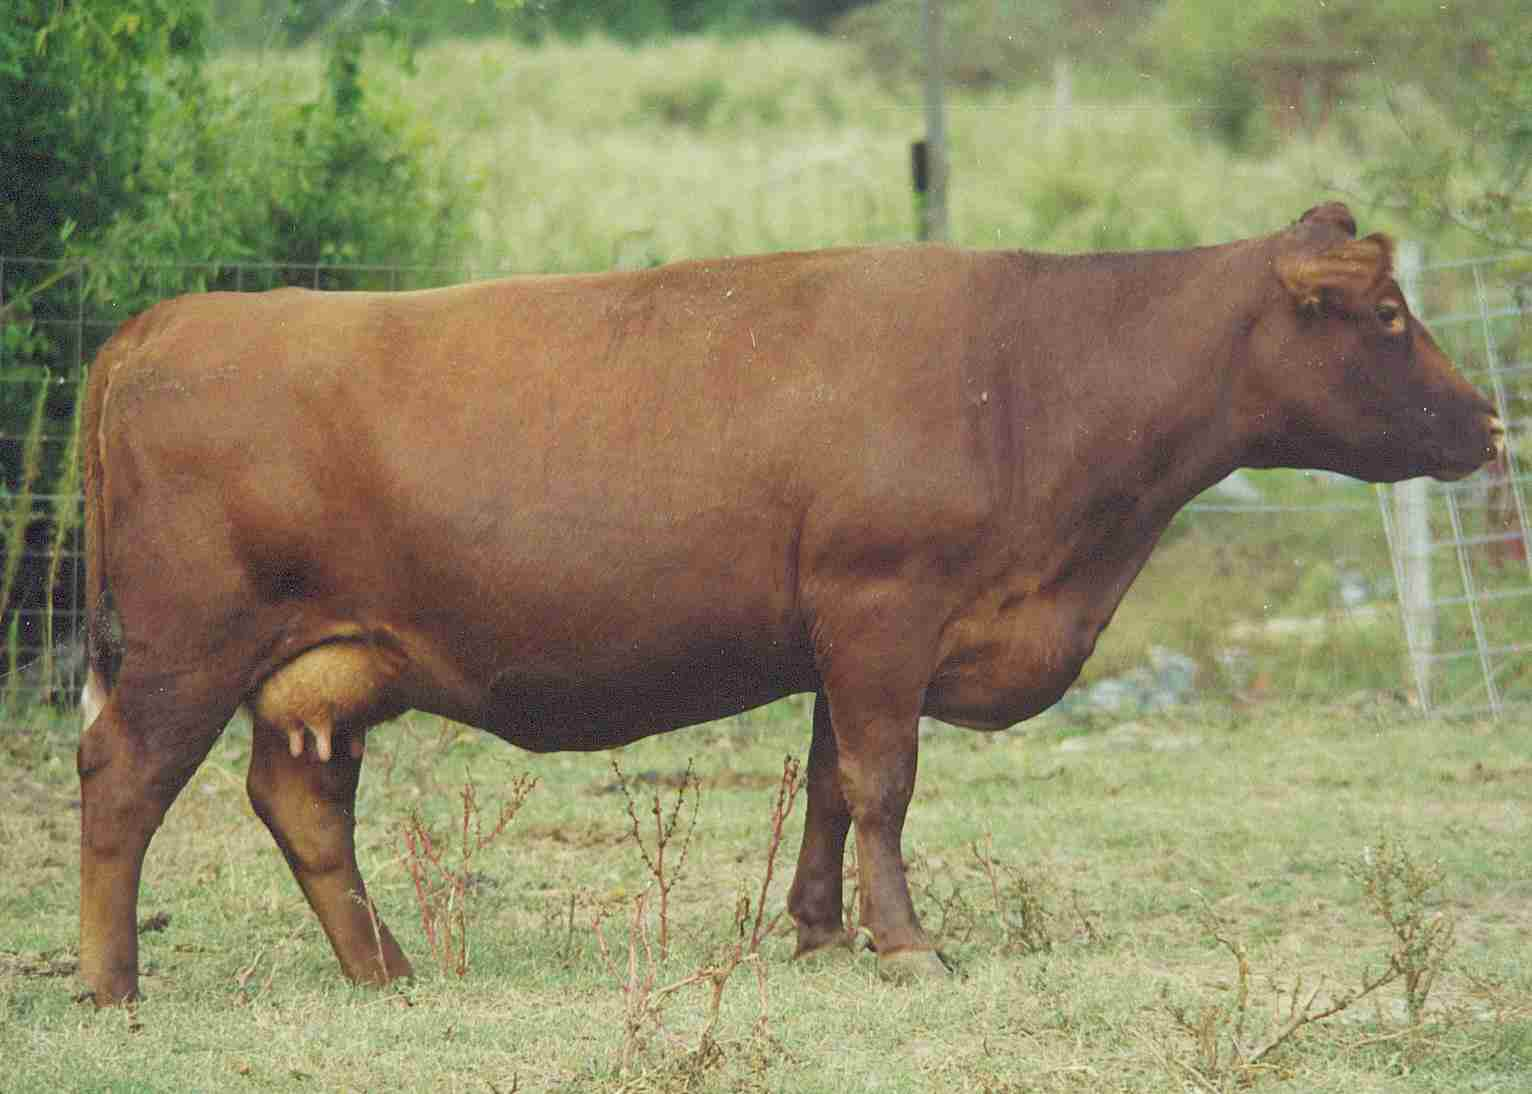
\includegraphics[width=\linewidth]{img/proof_cow.png}
      \end{column}

      \begin{column}{.45\linewidth}
        \begin{block}<2->{The Economist says:}
          \begin{itemize}
          \item Cows in Scotland are brown
          \end{itemize}
        \end{block}

        \begin{block}<3->{The Logician says:}
          \begin{itemize}
          \item No, no. There are cows in Scotland of which one is brown
          \end{itemize}
        \end{block}

        \begin{block}<4->{The Computer Scientist says:}
          \begin{itemize}
          \item No, no. There is at least one cow in Scotland of which one
            side is brown
          \end{itemize}
        \end{block}
      \end{column}
    \end{columns}
  \end{block}
\end{frame}
%%%%%%%%%%%%%%%%%%%%%%%%%%%%%%%%%%%%%%%%%%%%%%%%%%%%%%%%%%%%%%%%%%%%%%%%%%
\begin{frame}[squeeze]{Specification: Putting it into Practice}
  \begin{block}{Back to our Example: A sorting program}\smallskip
    \texttt{def sort(a:Array[Int]):Array[Int] = \{ \ldots\ \}}
  \end{block}\vspace{-.3\baselineskip}
  \begin{block}{Specification \only<4->{V1}}
    \begin{itemize}\vspace{-.2\baselineskip}
    \item \structure{Precondition}: $a$ is an array
    \item \structure{Post-condition}: returns the sorted argument array
    \item<2-> \alert{Is it good enough?}
      \only<3->{
         \alert{Not quite:} 
         \texttt{sort(\{2,1,2\} $\leadsto$ \{1,2,2,17\}} ~\Frownie}
    \end{itemize}
  \end{block}\vspace{-.8\baselineskip}
  \begin{block}<4->{Specification V2}
    \begin{itemize}\vspace{-.2\baselineskip}
    \item \structure{Precondition}: $a$ is an array
    \item \structure{Post-condition}: returns a sorted array \alert{with only
        elements} of $a$
    \item<5->[\Frownie] \texttt{sort(\{3,2,1\} $\leadsto$ \{2,2,2,2,2\}}
    \end{itemize}
  \end{block}\vspace{-.8\baselineskip}
  \begin{block}<6->{Specification V3}
    \begin{itemize}\vspace{-.2\baselineskip}
    \item \structure{Precondition}: $a$ is an array
    \item \structure{Post-condition}: returns a \alert{permutation} of $a$ that
      is sorted
    \item<7->[\Frownie] \texttt{sort(\{\})} leads to unwanted behavior
    \end{itemize}
  \end{block}\vspace{-.8\baselineskip}
  \begin{block}<8->{Specification V4}
    \begin{itemize}\vspace{-.2\baselineskip}
    \item \structure{Precondition}: $a$ is a \alert{non-null} array
    \item \structure{Post-condition}: returns a permutation of $a$ that
      is sorted
    \end{itemize}
  \end{block}
\end{frame}
%%%%%%%%%%%%%%%%%%%%%%%%%%%%%%%%%%%%%%%%%%%%%%%%%%%%%%%%%%%%%%%%%%%%%%%%%% 
\begin{frame}{The Contract Metaphor}
  \begin{boitequote}{B. Meyer, Computer 25(10)40-51, 1992}
    \hspace{-1.5em}\alert{Contract} is preferred specification metaphor for
    procedural and OO.
  \end{boitequote}\bigskip

  \begin{block}{Same Principles as \alert{Legal Contract} between a Client and
      Supplier}
    \begin{description}
    \item[Supplier] aka Implementer, in Java, a class or method
    \item[Client] Mostly a caller object, or human user for main()
    \item[Contract] One or more pairs of ensures/requires clauses\\
           defining mutual obligations of client and implementer
    \end{description}
  \end{block}

  \begin{block}{Meaning of a Contract: Specification of method \texttt{C@m()}}
    \begin{itemize}
    \item "If a caller of \texttt{C@m()} fulfills the \alert{required
        Precondition},\\ then the class \texttt{C} \alert{ensures} that the
      \alert{Postcondition} holds after \texttt{m()} finishes."
    \end{itemize}
  \end{block}
  \begin{block}{Wrong Interpretations:}
    \begin{itemize}
    \item "Any caller of C@m() must fulfill the required Precondition."
    \item "Whenever the required Precondition holds, then C@m() is executed."
    \end{itemize}
  \end{block}
\end{frame}
%%%%%%%%%%%%%%%%%%%%%%%%%%%%%%%%%%%%%%%%%%%%%%%%%%%%%%%%%%%%%%%%%%%%%%%%%%
\begin{frame}{What is Design By Contract?}
  \begin{boitequote}{}
    View the relationship between two classes as a formal agreement, expressing
    each party's rights and obligations.~\hfill{\rm -- Bertrand Meyer}
  \end{boitequote}

  \begin{block}{Example: Airline Reservation}
    \begin{tabular}{p{.15\linewidth}|p{.37\linewidth}|p{.37\linewidth}}\hline
      &Obligations&Rights\\\hline
      Customer&
      \begin{itemize}\vspace{-.8\baselineskip}
      \item Be at Paris airport at least 3 hour before scheduled departure time
      \item Bring acceptable baggage
      \item Pay ticket price
      \end{itemize}\vspace{-1.2\baselineskip}
      &
      \begin{itemize}\vspace{-.8\baselineskip}
      \item Reach Los Angeles
      \end{itemize}
      \\\hline
      Airline&
      \begin{itemize}\vspace{-.8\baselineskip}
      \item Bring customer to Los Angeles
      \end{itemize}
      &
      \begin{itemize}\vspace{-.8\baselineskip}
      \item No need to carry passenger who is late
      \item has unacceptable baggage
      \item or without paid ticket
      \end{itemize}\vspace{-1.2\baselineskip}
    \end{tabular}
  \end{block}
  \begin{itemize}
  \item Each party expects benefits (rights) and accepts obligations
  \item Usually, one party's benefits are the other party's obligations
  \item Contract is declarative: it is described so that both parties can
    understand \textit{what} service will be guaranteed without saying
    \textit{how}
  \end{itemize}
\end{frame}
%%%%%%%%%%%%%%%%%%%%%%%%%%%%%%%%%%%%%%%%%%%%%%%%%%%%%%%%%%%%%%%%%%%%%%%%%% 
\begin{frame}{Testing \textit{vs.} Verification}
  \begin{block}{Testing}
    \begin{itemize}
    \item \structure{Goal:} find evidence for \alert{presence} of failures
    \item \alert{Testing means to execute a program with the \textbf{intent of
          detecting failure}}
    \item \structure{Related techniques:}  code reviews, program inspections
    \item Automatize the testing process is delayed until the POO module
    \end{itemize}
  \end{block}

  \begin{block}{Verification}
    \begin{itemize}
    \item \structure{Goal:} find evidence for \alert{absence} of failures
    \item \alert{Testing cannot guarantee correctness, i.e., absence of
        failures}
    \item \structure{Related techniques:} code generation, program synthesis
      (from spec)
    \item<2->\alert{This week:} How can we prove the correctness of an algorithm?
    \end{itemize}
  \end{block}

  \begin{block}{Debugging}
    \begin{itemize}
    \item Systematic process to find and eliminate defects leading to
      observed failures
    \end{itemize}
  \end{block}
\end{frame}
%%%%%%%%%%%%%%%%%%%%%%%%%%%%%%%%%%%%%%%%%%%%%%%%%%%%%%%%%%%%%%%%%%%%%%%%%% 
\section{Hoare Logic}\sectionpage
%%%%%%%%%%%%%%%%%%%%%%%%%%%%%%%%%%%%%%%%%%%%%%%%%%%%%%%%%%%%%%%%%%%%%%%%%% 
\begin{frame}{Back on Hoare Logic}
  \begin{block}{Hoare Logic {\normalsize[Hoare 1969]}}
    \begin{itemize}
    \item Set of logical rules to reason about the correctness of computer
      programs
    \item \structure{Central feature:} description of state changes induced by
      code execution
    \item \alert{\textbf{Hoare triple:}} \framebox{$\{P\}~ C ~\{Q\}$}
      \begin{itemize}
      \item C is the code to be run
      \item P is the \alert{\textbf{precondition}}
        (assertion about previous state)
      \item Q is the \alert{\textbf{postcondition}}
        (assertion about next state)
      \item This can be read as ``If P is true, then when I run C, Q becomes
        true''
      \item C is said to satisfy specification $(P,Q)$
      \end{itemize}
    \item Such notation allows very precise algorithm specifications
    \item Axioms and Inference rules allow rigorous correctness demonstrations
      \smallskip
    \item \structure{Note:} other logics (temporal logic) proposed as
      replacement, but harder
    \end{itemize}
  \end{block}
  
  \begin{alertblock}{Game now}
    \begin{itemize}
    \item See how we can \textbf{prove} that a Hoare triple holds
    \end{itemize}    
  \end{alertblock}
\end{frame}
%%%%%%%%%%%%%%%%%%%%%%%%%%%%%%%%%%%%%%%%%%%%%%%%%%%%%%%%%%%%%%%%%%%%%%%%%% 
\begin{frame}{Assertions}
  \concept{What exactly is an assertion?}

  \begin{block}{Definition}\medskip
    Formula of first order logic describing relationships between algorithm's
    variables
  \end{block}

  \begin{block}{Constituted of:}
    \begin{itemize}
    \item \structure{Variables} of algorithm pseudo-code
    \item \structure{Logical connectors:} $\wedge$ (and) $\vee$ (or) $\neg$
      (not) $\Rightarrow$, $\Leftarrow$
    \item \structure{Quantifiers:} $\exists$ (exists), $\forall$ (for all)
    \item \structure{Value-specific elements} (describing integers, reals,
      booleans, arrays, sets, \ldots)
    \end{itemize}
  \end{block}

  \begin{block}{Example:}
    \begin{itemize}
    \item $(x\times y = z) ~\wedge~ (x\leq 0)$
    \item $n^2\geq x$
    \end{itemize}
  \end{block}
\end{frame}
%%%%%%%%%%%%%%%%%%%%%%%%%%%%%%%%%%%%%%%%%%%%%%%%%%%%%%%%%%%%%%%%%%%%%%%%%% 
\begin{frame}{Examples of specification}

  \begin{block}{Solving quadratic equations ($ax^2+bx+c=0$)}
    \begin{description}
    \item[P:] $a,b,c \in\mathbb{R}$ and $a\neq 0$
    \item[Q:] $(solAmount\in\mathbb{N}) \wedge (s,t \in\mathbb{R}) \wedge$\\
      ~~~$(~(solAmount = 0) \vee$\\
      ~~~~~$(solAmount = 1 \wedge as^2+bs+c=0) \vee$\\
      ~~~~~$(solAmount = 2 \wedge as^2+bs+c=0 \wedge at^2+bt+c=0 \wedge s\neq t)
      )$     
    \end{description}
  \end{block}

  \begin{block}{Possible implementation}
    
  \end{block}
  \begin{columns}
    \begin{column}{.4\linewidth}
  \framebox{
    \begin{minipage}{\linewidth}      
      $\Delta=b^2-4ac$\\
      if ($\Delta>0$) \\
      \null~~$s=\frac{-b+\sqrt{\Delta}}{2a}; t=\frac{-b-\sqrt{\Delta}}{2a};$\\
      \null~~$solAmount=2$\\
      else if ($\Delta=0$) \\
      \null~~$s=\frac{-b}{2a}; solAmount=1$\\
      else (ie, $\Delta<0$)\\
      \null~~solAmount=0
  \end{minipage}}      
    \end{column}

    \begin{column}{.5\linewidth}
      \begin{itemize}
      \item Here, the proof will be difficult\ldots
      \item \ldots because it is trivial.
      \item Correctness comes from definitions!
      \end{itemize}
    \end{column}
  \end{columns}
\end{frame}
%%%%%%%%%%%%%%%%%%%%%%%%%%%%%%%%%%%%%%%%%%%%%%%%%%%%%%%%%%%%%%%%%%%%%%%%%% 
\begin{frame}{Demonstration tool: inference rules}
  \begin{block}{Definitions}
    \begin{itemize}
    \item \structure{Inference:} deducting new facts by combining existing
      facts correctly
    \item \structure{Inference rule:} mechanism specifying how facts can be
      combined
    \end{itemize}
  \end{block}

  \begin{block}{Classical representation of each rule:}
    $$\frac{p_1, p_2, p_3, \ldots, p_n}{q}$$
    \begin{itemize}
    \item Can be read as ``if all $p_1, p_2, p_3, \ldots, p_n$ are true, then
      $q$ is also true''
    \item Or ``in order to prove $q$, you have to prove $p_1, p_2, p_3, \ldots,
      p_n$'' 
    \item Or ``$q$ can be deduced from $p_1, p_2, p_3, \ldots, p_n$''
    \end{itemize}
  \end{block}
\end{frame}
%%%%%%%%%%%%%%%%%%%%%%%%%%%%%%%%%%%%%%%%%%%%%%%%%%%%%%%%%%%%%%%%%%%%%%%%%% 
\begin{frame}{First axioms and rules}
  \begin{block}{Empty statement axiom}\vspace{-2\baselineskip}
    $$\frac{}{\{P\} skip \{P\}}$$
  \end{block}

  \begin{block}<+->{Assignment axiom}\vspace{-2\baselineskip}
    $$\frac{}{\{P[x/E]\} x:=E \{P\}}$$
    \begin{itemize}
    \item $P[x/E]$ is $P$ with all free occurrences of variable $x$ replaced
      with expression $E$
    \item \structure{Example:}
      \begin{itemize}
      \item \structure{P:} $x=a\wedge y=b$
      \item \structure{Q:} $x=b\wedge y=a$
      \item \structure{SWAP:} algorithm achieving transition; For example:
        $t=x; x=y; y=t$
      \item We should prove: $\{P\} SWAP \{Q\}$
      \end{itemize}
    \end{itemize}
  \end{block}

  \begin{block}<+->{Consequence rule}\vspace{-2\baselineskip}
    $$\frac{P'\Rightarrow P, \{P\} ~C~ \{Q\}, Q\Rightarrow Q'}{\{P'\} ~C~ \{Q'\}}$$    
    \begin{itemize}
    \item $P$ is said to be weaker than $P'$
    \item $Q$ is said to be stronger than $Q'$
    \end{itemize}
  \end{block}

\end{frame}
%%%%%%%%%%%%%%%%%%%%%%%%%%%%%%%%%%%%%%%%%%%%%%%%%%%%%%%%%%%%%%%%%%%%%%%%%% 
\begin{frame}{Rules for algorithmic constructs}
  \begin{block}<+->{Rule of composition}\vspace{-2\baselineskip}
    $$\frac{\{P\} C_1 \{Q\},~~ \{Q\} C_2 \{R\}}{\{P\} C_1;C_2 \{R\}}$$    
    \begin{itemize}
    \item   $C_1;C_2$ means that both code are executed one after the other.
    \item Can naturally be generalized to more than two codes
    \end{itemize}
  \end{block}

  \begin{block}<+->{Conditional Rule}\vspace{-2\baselineskip}
    $$~~~~\frac{\{P\wedge Cond\} ~T~ \{Q\},~~ P\wedge\neg Cond\Rightarrow Q}{\{P\} \mathbf{~if~} Cond \mathbf{~then~} T \mathbf{~endif~} \{Q\}}$$
  \end{block}

  \begin{block}<+->{Conditional Rule 2}\vspace{-2\baselineskip}
    $$~~~~~~~~~~\frac{\{P\wedge Cond\} ~T~ \{Q\},~~ \{P\wedge\neg Cond\} ~E~
      \{Q\}}{\{P\} \mathbf{~if~} Cond \mathbf{~then~} T \mathbf{~else~} E \mathbf{~endif~} \{Q\}}$$
  \end{block}

%  \begin{block}<+->{Loop Rule}\vspace{-2\baselineskip}
%    $$~~~~~~~~~~\frac{\{P\wedge Cond\} ~T~ \{Q\},~~ \{P\wedge\neg Cond\} ~E~
%      \{Q\}}{\{P\} \mathbf{~if~} Cond \mathbf{~then~} T \mathbf{~else~} E \mathbf{~endif~} \{Q\}}$$
%  \end{block}

  \begin{block}<+->{While Rule}\vspace{-2\baselineskip}
    $$\frac{\{I\wedge Cond\} ~L~ \{I\}}
            {\{I\} \mathbf{~while~} Cond \mathbf{~do~} 
                   L \mathbf{~done~} \{I\wedge\neg Cond\}}$$
    \begin{itemize}\vspace{-.5\baselineskip}
    \item $\{I\}$ is said to be the \alert{\textbf{loop invariant}}
    \end{itemize}
  \end{block}
\end{frame}
%%%%%%%%%%%%%%%%%%%%%%%%%%%%%%%%%%%%%%%%%%%%%%%%%%%%%%%%%%%%%%%%%%%%%%%%%% 
\begin{frame}{How to prove algorithms?}
  \begin{block}{The two things to prove about algorithms}
    \begin{itemize}
    \item \structure{Correction proof:}
      when it terminates, the algorithm produce a valid result\\
      {\small with regard to problem specification}
    \item \structure{Termination proof:} the algorithm always terminate
    \end{itemize}
  \end{block}
  \begin{block}{There is no perfect proof, only good ones}
    \begin{itemize}
    \item Your main goal is to \textbf{convince} people that your code works
    \item If your friends are permissive, very sparse hints may be enough
    \item If your friends are picky, you need to provide more details
    \item Note that I'm gonna be very picky in exam ;)
    \end{itemize}
  \end{block}
  \begin{block}{Detailed proofs}
    \begin{itemize}
    \item Most convinient way to prove an algorithm in practice: think backward
    \item Compute the weakest precondition you need to get the postcondition you
      want
    \item What must be the precondition of the given code to get the
        wanted postcondition?
    \end{itemize}
  \end{block}
\end{frame}
%%%%%%%%%%%%%%%%%%%%%%%%%%%%%%%%%%%%%%%%%%%%%%%%%%%%%%%%%%%%%%%%%%%%%%%%%%%%%%
\newcommand{\WP}[1]{\textbf{WP}($#1$)}
\begin{frame}{Computing the Weakest Preconditions}
  \begin{block}{Computing the WP to get the post-condition \{Q\}
      from C -- WP(C,Q)}
    \begin{enumerate}
\item \WP{nop, Q}  $\equiv Q$
\item \WP{x:=E, Q} $\equiv Q[x:=E]$
\item \WP{C;D, Q}  $\equiv$ \WP{C, \WP{D,Q}}
\item \textbf{WP}(\texttt{if} $Cond$ \texttt{then} $C$ \texttt{else} $D$, Q)
  $\equiv (Cond=\mathtt{true}\Rightarrow \mathbf{WP}(C,Q))~\wedge~
          (Cond=\mathtt{false}\Rightarrow \mathbf{WP}(D,Q))$
\item \textbf{WP}(\texttt{while} $E$ \texttt{do} $C$ \texttt{done} ,Q) %\{inv I var V\}
  $\equiv I$ \hfill (with I invariant, V variant)\\
  Plus the following proof obligations:
  \begin{itemize}
  \item[$\bullet$] $(E=\mathtt{true}\wedge I\wedge V=z) \Rightarrow
    \mathbf{WP}(C,I\wedge V<z))$
    \hfill(variant gets decremented)
  \item[$\bullet$] $I\Rightarrow V\geq 0$
    % 
    \hfill (variant remains valid)
  \item[$\bullet$] $(E=\mathtt{false}\wedge I) \Rightarrow Q$
    %
    \hfill (once done, Q is achieved)
  \end{itemize}
\end{enumerate}

  \end{block}

  \begin{block}{Seems complicated, but isn't that much}
    \begin{itemize}
    \item The process is automated enough to keep quite mecanical and simple
    \item We'll come back on this in lab (and exam ;)
    \end{itemize}
  \end{block}
\end{frame}
%%%%%%%%%%%%%%%%%%%%%%%%%%%%%%%%%%%%%%%%%%%%%%%%%%%%%%%%%%%%%%%%%%%%%%%%%%%%%%
\section{Proving Recursive Functions}\sectionpage
%%%%%%%%%%%%%%%%%%%%%%%%%%%%%%%%%%%%%%%%%%%%%%%%%%%%%%%%%%%%%%%%%%%%%%%%%%%%%%

\begin{frame}{Idea of the correction of recursive function}

  \structure{$P(n)$}: Precondition at step $n$; \structure{$Q(n,r_n)$}:
  Postcondition at step $n$ with result $r_n$%\vspace{-\baselineskip}

  \bigskip
  \centerline{\textbf{\alert{We want to show \framebox{${P(n) \:\{TREC\}\: Q(n,r_n)}$}}}}
  \bigskip

  \centerline{%
    \includegraphics<1| handout:0>[subfig=1]{fig/proof-recursion.fig}%
    \includegraphics<2| handout:0>[subfig=2]{fig/proof-recursion.fig}%
    \includegraphics<3| handout:0>[subfig=3]{fig/proof-recursion.fig}%
    \includegraphics<4| handout:1>[subfig=4]{fig/proof-recursion.fig}%
  }%
  \bigskip

  \uncover<2->{
  If $f(n)$ is expressed as function of $f(n-1)$, we need:
    \begin{itemize}
    \item In \structure{recursive case}
      \begin{itemize}
      \item Precondition of $f(n)$ implies precondition of $f(n-1)$ 
        \hfill\alert{\textcircled{\scriptsize 1}~~}\\      
        {\footnotesize If not, the computation is impossible}
      \uncover<4->{
      \item Hyp: postcondition of $f(n-1)$ true. Proof postcondition of
        $f(n)$\hfill~\alert{\textcircled{\scriptsize 3}}
      }
  
      \end{itemize}
    \uncover<3->{
    \item In \structure{base case}
      \begin{itemize}
      \item precondition and computation allow to prove postcondition
        \hfill\alert{\textcircled{\scriptsize 2}~~}
      \end{itemize}      
    }
    \end{itemize}
  }
\end{frame}

%%%%%%%%%%%%%%%%%%%%%%%%%%%%%%%%%%%%%%%%%%%%%%%%%%%%%%%%%%%%%%%%%%%%%%%%%%%%%%
% \begin{frame}{Proof of correctness (1/2)}
  
%   \hfill\alert{$P(n) \:\{TREC\}\: Q(n,r_n)$\hfill$(1)$}\\[.2\baselineskip]
%   \hfill\small{$P(n) \:\{\text{\textbf{if} cond \textbf{then} \textsc{tter} \textbf{else} \textsc{tgen}}\}\: Q(n,r_n)$}\hfill~
  

%   \bigskip\bigskip

%   \begin{columns}[t]
%     \begin{column}{.6\linewidth}
%     \uncover<2->{
%       \structure{\large Simple case}: \textsc{tgen} and \textsc{tter} are affectations\\[.2\baselineskip]
      

%       \begin{description}
%       \item[TGEN:] $r\leftarrow G(n,f(n_{int}))$
%       \item[TTER:] $r\leftarrow v(n)$
%       \end{description}     
%     }
 
%     \uncover<3->{
%       \structure{With}%\vspace{-1.45\baselineskip}
%       \begin{description}
%       \item[$n_{int}$] Value of recursive call
%       \item[$f(x)$] The recursive call
%       \item[$v(n)$] Function w/o call to $f(n)$
%       \item[$G(n,y)$] Function:
%         \begin{itemize}
%         \item W/O recursive call to $f(n)$
%         \item Defined  $\forall n\text{ parameter},\forall y$
%         \end{itemize}
%       \end{description}
%     }
%     \end{column}


%     \uncover<4->{
%     \begin{column}{.4\linewidth}
%       \structure{\large Example}: Factorial
%       \begin{description}
%       \item[TGEN:] $r\leftarrow n\times facto(n-1)$
%       \item[TTER:] $r\leftarrow 1$
%       \end{description}     
%       ~\\
%       \begin{description}
%       \item[$n_{int}$] $=n-1$
%       \item[$f(x)$]: $facto(x)$
%       \item[v(n)] $=1$
%       \item[G(n,y)] $=n\times y$
%     }

%         \medskip
%     \uncover<5->{
%       \item[$P(n)$]: $n\geq 0$
%       \item[$Q(n,r)$]: $r=n!$
%       \item[cond(n)]: n=0 
%       \end{description}
%     \end{column}
%     }
%   \end{columns}
  
% \end{frame}
%%%%%%%%%%%%%%%%%%%%%%%%%%%%%%%%%%%%%%%%%%%%%%%%%%%%%%%%%%%%%%%%%%%%%%%%%%%%%%
% \begin{frame}{Proof of correctness}

%   \concept{\fbox{$P(n) \:\{TREC\}\: Q(n,r_n)$}}


%   \structure{\Large Simple case: }{\large \textsc{tter} and \textsc{tgen} are affectations}
%   \begin{itemize}
%   \item \structure{\large Algorithm computing
%       $r=f(n)$}
%     \begin{tabbing}
%       \textbf{if} cond(n) \=\textbf{else} \=$r\leftarrow v(x)$\kill
%       \textbf{if} cond(n) \>\textbf{then} \>$r\leftarrow v(x)$\\
%       \>\textbf{else}\>$r\leftarrow G(n,f(n_{int}))$
%     \end{tabbing}

%   \item \structure{\large To prove , it is sufficient to prove:}
%     \begin{itemize}
%     \item In \structure{terminal case}: precondition and computation imply postcondition

%       \centerline{\alert{$P(n)\wedge cond(n) \Rightarrow Q(n,r)$}}
%     \item In \structure{general case}:
%       \begin{itemize}
%       \item \structure{Recursive descent}: precondition of $f(n)$ implies
%         precondition of $f(n-1)$

%         \centerline{\alert{$P(n)\wedge\neg cond(n)\Rightarrow P(n_{int})$}}
%       \item \structure{Recursive Climb}: postcondition of $f(n-1)$ implies
%         postcondition of $f(n)$
        
%         \centerline{\alert{$P(n)\wedge\neg cond(n)\wedge Q(n_{int},r_{int})
%             \Rightarrow Q(n,r)$}}
%       \end{itemize}          
%     \end{itemize}
%   \end{itemize}

%   \uncover<2->{
%     \vspace{\baselineskip}
%     \structure{\Large General Case: }{\large harder}
%     \begin{itemize}
%     \item You need to combine with the proofs of the previous section
      
%       \hfill$P(x)\Rightarrow P(x_{int})$
%       \hfill$Q(x_{int},r_{int})\Rightarrow Q(x,r)$
%       \hfill~
%     \end{itemize}
%   }
% \end{frame}
%%%%%%%%%%%%%%%%%%%%%%%%%%%%%%%%%%%%%%%%%%%%%%%%%%%%%%%%%%%%%%%%%%%%%%%%%%%%%% 
\begin{frame}{Example of the factorial (how unexpected)}
  \begin{columns}
    \begin{column}{.78\textwidth}
      \DontPrintSemicolon\SetAlgoLined
      \AlgoDontDisplayBlockMarkers\SetAlgoNoEnd

      \SetKwFunction{Factorial}{factorial}

      \SetKwProg{Fn}{Function}{ is}{}
      \Fn{factorial(n)}{
        \uIf{\alert<5>{n == 0}}{
          \alert<5>{\Return 1} \tcc*{base case}
        }
        \Else{
          \Return{n $\times$ \Factorial{n-1}\tcc*{recursive case}}
        }
      }
    \end{column}
  \end{columns}

  \medskip

  ~\hfill
  \structure{$P(n)$}: $n\geq 0$\hfill
  \structure{cond(n)}: $n=0$\hfill
  \structure{$Q(n,r)$}: $r=n!$\hfill
  \structure{$n_{int}$}= $n-1$\hfill~
  \bigskip

  \begin{itemize}
  \item \structure{Descent:}
    \alert{$P(n)\wedge\neg cond(n)\Rightarrow P(n_{int})$}
    \uncover<2->{$\equiv (n\geq 0)\wedge (n\neq 0)\Rightarrow (n-1\geq 0)$}

    \uncover<3->{Trivial}
  \item \structure{Base Case}:
    $\alert{P(n)\wedge cond(n) \Rightarrow Q(n,r)}
    \uncover<4->{\equiv n\geq 0\wedge n=0\Rightarrow r=n!}$ % FIXME SUR CETTE LIGNE

    \uncover<5->{True (since $1=0!$ no matter what happens -- look at the base
      case's code)}

  \item \structure{Recursive climb:}
    $\alert{P(n)\wedge\neg cond(n)\wedge Q(n_{int},r_{int}) \Rightarrow Q(n,r)}$

    $\uncover<6->{\equiv(n\geq 0)\wedge (n\neq 0)\wedge (r_{int}=n_{int}!) \Rightarrow (r=n!)}$

    \medskip
    \uncover<7->{
      True because:
      \begin{itemize}
      \item $r=n\times r_{int}$ in general case (by \textit{looking at the
          code})
      \item $r_{int}=n_{int}!=(n-1)!$ by induction hypothesis
      \item $r=n\times (n-1)!=n!$
      \end{itemize}
    }   
  \end{itemize}
\end{frame}

%%%%%%%%%%%%%%%%%%%%%%%%%%%%%%%%%%%%%%%%%%%%%%%%%%%%%%%%%%%%%%%%%%%%%%%%%%%%%% 
\begin{frame}{Proof of Termination}
  \begin{itemize}
  \item \structure{Sufficient Conditions}:
    \begin{itemize}
    \item Successive values of parameter $x$: \alert{strictly monotonous suite}\\ 
      (may need to specify the order)
    \item Existence of an \alert{extrema} $x_0$ \alert{verifying the
        stopping condition}
    \end{itemize}
  \item \structure{Remarque}: that's no necessary condition\\
    The \hyperlink{syracuse}{Syracuse suite} seems to terminate without
    this\bigskip

  \uncover<2>{
  \item \structure{Example:} the factorial, of course
    \begin{itemize}
    \item $n\geq 0$
    \item n strictly decreasing
    \item 0 = stopping condition
    \end{itemize}
  }
  \end{itemize}
\end{frame}
%%%%%%%%%%%%%%%%%%%%%%%%%%%%%%%%%%%%%%%%%%%%%%%%%%%%%%%%%%%%%%%%%%%%%%%%%%%%%
\section{Conclusion}\sectionpage
\begin{frame}{The dark side of Software Correctness Proofs}
  \begin{block}{Being picky can lead to long proofs}
    \begin{itemize}
    \item Lot and lot of mathematical work to prove even simple algorithms
    \item Overly detailed proofs are done only when really needed: \\
      {\small Aircraft, Nuclear power plant, Emergency room, \ldots}
    \item But that's not impossible; One success story amongst hundreds:\\
      {\small SACEM embedded system controling the train speed on
        the RER Line A in Paris.} 
    \end{itemize}
  \end{block}
  \begin{block}{Support from language / automated tools would be welcomed}
    \begin{itemize}
    \item Unfortunately, Java/Scala is not Ada (or even better: Eiffel)
    \item Java solution (JML -- Java Modeling Language): far from production
      ready
    \item Scala is better regarding algorithms' specification, but still a
      moving target
    \end{itemize}
  \end{block}
\end{frame}

\begin{frame}{The bright side of Software Correctness Proofs}
  \begin{block}{Sometimes you \alert{have to} prove your code}
    \begin{itemize}
    \item \structure{Cost/gain ratio}: if you cannot afford to loose, prove it correct
      {\small (nuclear plants)}
    \item If your client wants proofs, the competitors disappear
      {\small(competitive advantage)}
    \item You're studying in Nancy, there is a local history of algorithm proofs
    \item There will be 1/4 of points on proofs at the exam \ldots
    \end{itemize}
  \end{block}\vspace{-.2\baselineskip}

  \begin{block}{Proofs are useful even when it is not mandatory}
    \begin{itemize}
    \item Expressing pre/post and loop invariant greatly helps understanding the code
    \item This understanding helps writing the right test cases
    \item And tests are not overly pleasant either (you'll see in POO!)
    \end{itemize}
  \end{block}\vspace{-.2\baselineskip}

  \begin{block}{What is expected for the exam}
    \begin{itemize}
    \item Well, that's similar to when you write code
    \item I don't bother a missing \} in the code, as long as the idea is here
    \item I don't bother a partially wrong proof, as long as the method is here
    \end{itemize}
  \end{block}\vspace{-.5\baselineskip}

  \begin{flushright}
    (this ends the third lecture)    
  \end{flushright}

\end{frame}
% LocalWords:  Hoare LocalWords postcondition
%% coding: utf-8
